
 \documentclass{article}
 \usepackage{amsmath}
 \usepackage{graphicx}
 \usepackage{float}
 \usepackage{listings}
 \lstset{language=Matlab,basicstyle=\ttfamily}
 \title{\textsf{MapleTex}: Embedding \textsf{Maple} Results in \LaTeX\ Documents\\ {\small version 2022.02.05}}
 \author{Athanasios Kehagias\\ \texttt{kehagiat@ece.auth.gr}}
 \setlength{\textwidth}{6.75in}
 \setlength{\textheight}{9.00in}
 \setlength{\oddsidemargin}{0 in}
 \setlength{\topmargin}{0 in}
 \begin{document}
 \maketitle
 \section{Introduction}
 \textsf{MapleTex} is a \emph{very simple} package
 \footnote{Essentially a single script.}
 intended to enable the user to \emph{programmatically} 
 include the results of \textsf{Maple} computations in \LaTeX\  documents;
 the focus is on \emph{symbolic} computations but numerics and figures can also be used. 
 Hence it is similar to the various ``sweave'' packages that exist for \textsf{Matlab},
 \textsf{SageMath}, \textsf{R}, \textsf{Python} etc. But the emphasis of \textsf{MapleTex} 
 is on \emph{simplicity}.
 \footnote{Further discussion of this point appears in the Postscript.}
 
 \section{Installation}
 Simply unzip the file \texttt{MapleTex.zip} into some folder. 
 The basic files are \texttt{MapleTex.mw} and \texttt{MapleTex.mpl}. The first is a worksheet which 
 sets some variables and invokes the second, a script (collection of \textsf{Maple} commands) 
 which performs the substitutions contained in your own (mixed \textsf{Maple}/\LaTeX) script.
 Additional files are \texttt{MapleTexDoc.pdf} (the current document) and \texttt{MapleTexDoc.mpl} 
 (the mixed \textsf{Maple}/\LaTeX\  script which produced \texttt{MapleTexDoc.pdf}). 
  
 To run \textsf{MapleTex} you must have (obviously) installed \textsf{Maple} and a \TeX\  distribution. 
 I have tested \textsf{MapleTex} with \textsf{Maple 2018} and \textsf{TeX Live 2019} on
 \textsf{Windows 7, 10, 11}. Since it only depends on \textsf{Maple} and \LaTeX,
 it will probably work fine on \textsf{Linux} and \textsf{Apple} operating systems,
 but I have not tested this. 
 
 \section{QuickStart}
 Execute (in \textsf{Maple}) the worksheet \texttt{MapleTexDoc.mw}. You will get the files \texttt{MapleTexDoc.tex} 
 and \texttt{MapleTexDoc.pdf} (the current file).
 Open \texttt{MapleTexDoc.mpl}  to see the code which produced the document
 (some of the code is explained in a later section). 
 
 \section{Usage}
 The \textsf{MapleTex} workflow is as follows. 
 \begin{enumerate}
 \item Write a \emph{single} \textsf{Maple} script, e.g., \texttt{foo.mpl}, 
 which contains both \textsf{Maple} commands and \LaTeX\  code (embedded as comments);
 the \LaTeX\  code can include the control word \texttt{latex(a)}, where \texttt{a}, 
 is a \textsf{Maple} variable (details will be given a little later).     
 \item The file \texttt{foo.m} must be created in the same folder which contains \texttt{MapleTex.m}.
 \item Open (in \textsf{Maple}) the worksheet \texttt{MapleTex} and substititute 
 \texttt{fn:="MapleTexDoc":} with \texttt{fn:="foo":} 
 \item Run the the worksheet; when execution is completed you have the following files.
 \begin{enumerate}  
 \item \texttt{foo.tex}: your \LaTeX\  code with \textsf{Maple} results having replaced
 the \texttt{latex(a)} and \texttt{figur(b)} control words.
 \item \texttt{foo.pdf}: the output of \texttt{foo.tex} as compiled by \textsf{pdflatex}.
 \end{enumerate}
 \end{enumerate}

 \noindent To use \textsf{MapleTex} follow the above workflow.
 The file \texttt{foo.mpl} must be created in the same folder where you unzipped \texttt{Mapletex.zip}. The rules for writing 
 \textsf{MapleTex} files are as follows.
 \begin{enumerate}
 \item Each line contains either \emph{only} \textsf{Maple} code  or \emph{only} \LaTeX\ code. 
 \item \textsf{Maple} code is written as usual.
 \item \LaTeX\ code is also written as usual with the following two exceptions. 
 \begin{enumerate}
 \item Every line of \LaTeX\ code is preceded by the characters \texttt{\#\#} (so, as far as \textsf{Maple} 
 is concerned, these
 are comment lines).
 \item You can use the additional command \texttt{latex(\;)} (entered in \LaTeX\ code \textbf{without} a backslash!). 
 Every occurrence of \texttt{latex(a)} in the \LaTeX\  part of your code will be replaced by the \LaTeX\ expression for
  \texttt{a}, where it is assumed that \texttt{a} has been defined in the \textsf{Maple} part of your code.
 \end{enumerate}  
 \item In addition you must obey the following two rules.
 \begin{enumerate}
 \item The first line of \texttt{foo.mpl} must be \texttt{VARS:=[]:}.
 \item The last line of every block of \textsf{Maple} code must have the form \texttt{VARS:=[op(VARS),"a","b"]}
 where \texttt{"a"}, \texttt{"b"} etc. are variables which you want to use for \LaTeX\ substitutions.
 For example
 \begin{lstlisting}
 with(LinearAlgebra):
 C:=Matrix([[a,b],[c,d]]):
 CI:=MatrixInverse(C):
 VARS:=[op(VARS),"C","CI"]:
 \end{lstlisting}
 \end{enumerate}  
 \end{enumerate}  

 \section{Some Examples and Explanations}
 Let us now look at some parts of \texttt{MapleTexDoc.mpl}.
 \begin{enumerate}
 \item The file  starts with the lines 
 \begin{lstlisting}
 ## \documentclass{article}
 ## \usepackage{amsmath}
 ## \usepackage{graphicx}
 \end{lstlisting}
 and continues like this with typical \LaTeX\ preamble commands. Note that, since these are 
 \LaTeX\ commands, they are preceded by \texttt{\#\#}.
 \item After a while we have  the lines 
 \begin{lstlisting}
 ## \begin{document}
 ## \maketitle
 ## \section{Introduction}
 ## \texttt{MapleTex.m} is a \emph{very simple} script intended to 
 ## implement \emph{literate programming} in \textsf{Maple}. 
 \end{lstlisting}
 and so on, where we write our \LaTeX\ content as usual, but always using the \texttt{\#\#} line prefix.
 \item Things get more interesting when we introduce symbolic computations. So for example the code 
 \begin{lstlisting}
 ft0:=t*exp(t):
 Derft0:=Diff(ft0,t):
 derft0:=diff(ft0,t):
 Intft0:=Int(ft0,t):
 intft0:=int(ft0,t):
 VARS:=[op(VARS),"ft0","Derft0","derft0","Intft0","intft0"]:
 ## \item Let us compute the derivative and the indefinite integral 
 ## of \(f(t)=latex (ft0)\). They are
 ## \[
 ## latex (Derft0)=latex (derft0) \qquad \text{and} 
 ## \qquad latex (Intft0)=latex (intft0). 
 ## \]
 \end{lstlisting}
 produces the following results:

 \qquad Let us compute the derivative and the indefinite integral 
 of \(f(t)=t{{\rm e}^{t}}\). They are
 \[
 {\frac {\rm d}{{\rm d}t}} \left( t{{\rm e}^{t}} \right) ={{\rm e}^{t}}+t{{\rm e}^{t}} \qquad \text{and} \qquad \int \!t{{\rm e}^{t}}\,{\rm d}t= \left( t-1 \right) {{\rm e}^{t}}. 
 \]
 Similarly,  the code
 \begin{lstlisting}
 g:=1/n^2:
 G1:=Sum(g,n=1..infinity):
 G2:=sum(g,n=1..infinity):
 G0:=evalf(G2):
 VARS:=[op(VARS),"g","G1","G2","G0"]:
 ## \qquad Let us write the sum of \(g(n)=latex (g)\), i.e., 
 ## \(latex (G1)  = latex (G2) = latex (G0)\).
 \end{lstlisting}
 produces the following results

 \qquad Let us write the sum of \(g(n)={n}^{-2}\), i.e., 
 \(\sum _{n=1}^{\infty }{n}^{-2}  = 1/6\,{\pi}^{2} =  1.644934068\).
 \item Here is an example on how to include figures. Suppose you want to plot a sinusoid;
 you can use the following code in \texttt{foo.mpl}. 
 \begin{lstlisting}
 p1:=plot(sin(3*x),x=0..2*Pi):
 plotsetup(png, plotoutput = "FIG001"):
 print(p1):
 ## \begin{figure}[H]
 ## \centering
 ## 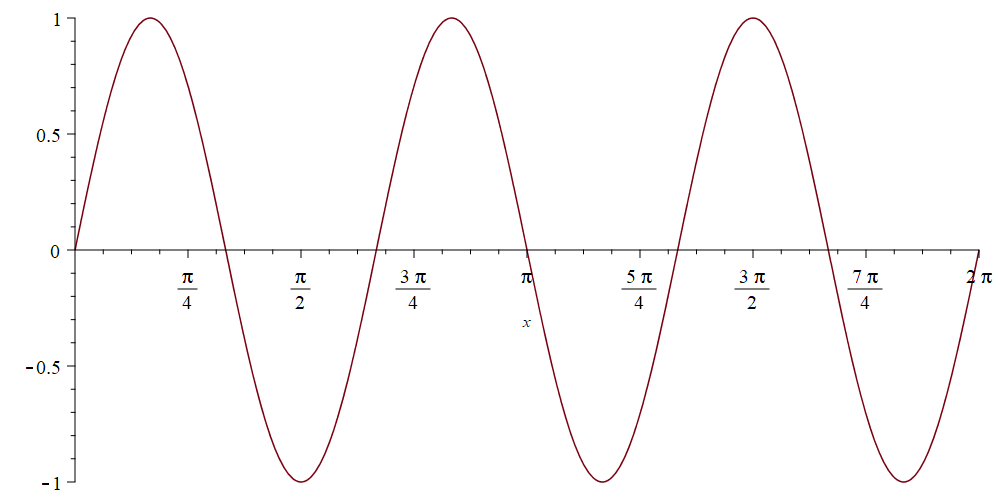
\includegraphics[scale=0.2]{FIG001}
 ## \caption{A plot of \(F(x)=\sin(3x)\).}  \label{FIG001}
 ## \end{figure}
 \end{lstlisting}
 The first line of the above fragment creates a plot object, the second one  sets the plot output 
 to be the file \texttt{FIG001.png} 
 \footnote{Various \texttt{plotoptions} can be included; see the \textsf{Maple} documentation
 on \texttt{plotsetup}.}
 and the third prints the plot \texttt{p1} to \texttt{FIG001.pdf}.
 The remaining five lines are ``regular'' \LaTeX\ code which includes the figure in the \LaTeX\ document.
 This results in the following plot 
 \begin{figure}[H]
 \centering
 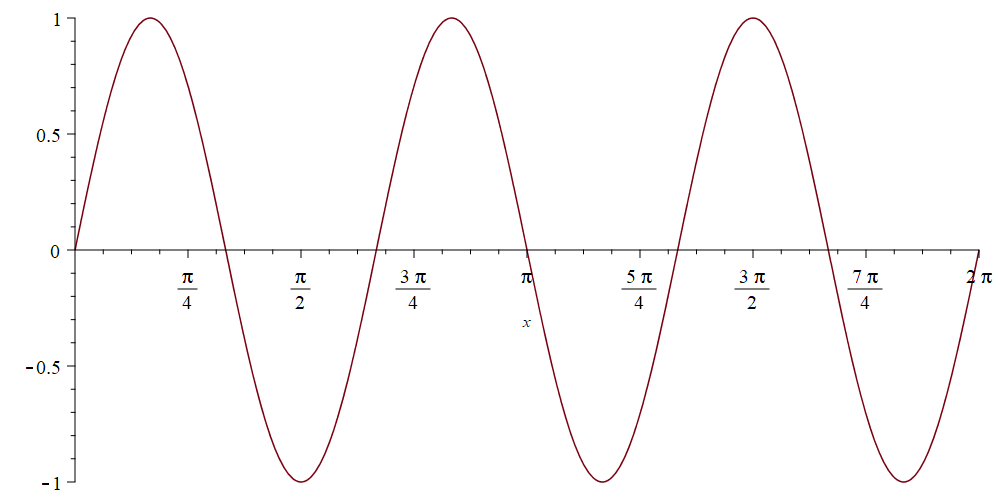
\includegraphics[scale=0.2]{FIG001}
 \caption{A plot of \(F(x)=\sin(3x)\).}  \label{FIG001}
 \end{figure}
 \item Let us now present  some additional symbolic results. To see the code which
 generates the following lines open \textsf{MapleTexDoc.mpl} and look at around lines 191-275.
 \begin{enumerate}
 \item Let us solve the equation
 \[
 {x}^{2}+x+1=0. 
 \]
 The solution is
 \[
 x_1=-1/2+i/2\sqrt {3} \qquad \text{and} \qquad x_2=-1/2-i/2\sqrt {3}.  
 \]
 \item Now let us solve the differential equation
 \[
 {\frac {{\rm d}^{2}}{{\rm d}{t}^{2}}}f \left( t \right) -3\,{\frac {\rm d}{{\rm d}t}}f \left( t \right) +2\,f \left( t \right) ={{\rm e}^{3\,t}} \text{ with } f \left( 0 \right) ={\rm e} \text{ and } \mbox {D} \left( f \right)  \left( 0 \right) ={\rm e} 
 \]
 The solution is
 \[
 f(t)= \left( 1/2\, \left( {{\rm e}^{t}} \right) ^{2}-{{\rm e}^{t}}+{\rm e}+1/2 \right) {{\rm e}^{t}} 
 \]
 \item Next let us solve the integral equation
 \[
 \int_{0}^{t}\!x \left( s \right) {{\rm e}^{t-s}}\,{\rm d}s=\sin \left( t \right) . 
 \]
 The solution is
 \[
 x(t)=\cos \left( t \right) -\sin \left( t \right)  
 \]
 \item The Taylor series of \(f(x)={\frac {{{\rm e}^{x}}}{x+1}}\) is
 \[
 1+1/2\,{x}^{2}-1/3\,{x}^{3}+3/8\,{x}^{4}-{\frac {11\,{x}^{5}}{30}}
 \]
 \item We can do integral transforms. The Fourier transform of \(f(t)= \left( {t}^{2}+1 \right) ^{-1}\) is
 \[
 F(w)=\pi\, \left( {{\rm e}^{-w}}{\it Heaviside} \left( w \right) +{{\rm e}^{w}}{\it Heaviside} \left( -w \right)  \right) 
 \]
 and the inverse Laplace transform of \(F(s)={\frac {s+1}{{s}^{2}+s+1}}\) is
 \[
 f(t)=1/3\,{{\rm e}^{-t/2}} \left( 3\,\cos \left( 1/2\,\sqrt {3}t \right) +\sqrt {3}\sin \left( 1/2\,\sqrt {3}t \right)  \right) 
 \]
 \item We define a matrix and compute its powers
 \[
 C= \left[ \begin {array}{cc} a&b\\ \noalign{\medskip}c&d\end {array} \right] , \qquad C^2= \left[ \begin {array}{cc} {a}^{2}+bc&ab+bd\\ \noalign{\medskip}ca+dc&bc+{d}^{2}\end {array} \right] , \qquad C^{-1}= \left[ \begin {array}{cc} {\frac {d}{ad-bc}}&-{\frac {b}{ad-bc}}\\ \noalign{\medskip}-{\frac {c}{ad-bc}}&{\frac {a}{ad-bc}}\end {array} \right] .
 \]
 \item We can also insert 3D figures such as the following.
 \begin{figure}[H]
 \centering
 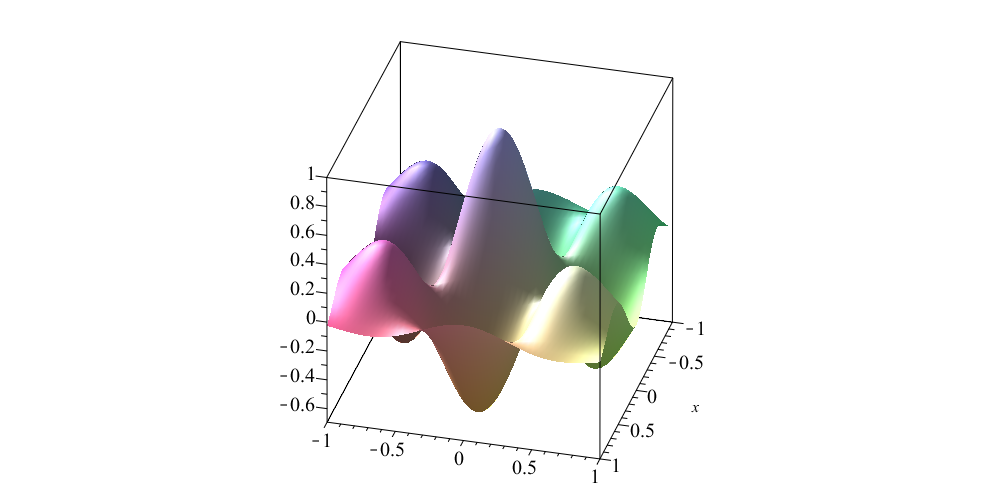
\includegraphics[scale=0.4]{FIG002}
 \caption{A plot of \(G(x,y)=e^{-(x^2+y^2)}\cos(ax)\cos(by)\).}  \label{FIG002}
 \end{figure}
 
 \end{enumerate}
 \end{enumerate}
 
 \section{Postscript}
 My motivation for writing \textsf{MapleTex} was the need for a simple system to create problem sets and exams 
 (and answers!) for my math classes. I have been using several computer algebra systems: 
 \textsf{Maple}, \textsf{SageMath}, \textsf{SymPy},
 the symbolic math toolboxes of \textsf{Matlab} and \textsf{Octave},  and so on.
 Not wanting to reinvent the wheel I looked at what was available. I started with \textsf{SageTex}; alas, I was
 never able to properly install and run it. I tried several additional packages and I found each one either 
 too confusing to set up, or not providing the functionalities I wanted, or both.
 
 Consequently I decided to write my own package. I am a simple guy and \textsf{MapleLaTex} is a simple hack. 
 I am certain that any sufficiently interested serious programmer can produce a much better version
 and I will be very happy if someone does. 
 In the meantime, \textsf{MapleTex} works  right out of the box and does what I want it to do: 
 programmatically incorporate \textsf{Maple} results into my \LaTeX\  documents. 
 
 In conclusion, there are a few improvements / extensions on which I hope to work in the future. I list them 
 in order of decreasing priority. 
 \begin{enumerate}
 \item Automatic generation of a list of substitutions. Currently this has to be provided by the user
 (this is the role of the \texttt{VARS:=[op(VARS),"a","b"]} commands). I was looking for a \textsf{Maple} command 
 which generates the list of all workspace variables (something like \texttt{whois} in \textsf{Matlab})
 but I could not find it; any help will be appreciated.
 \item In the current implementation, variable names cannot be ``reused''. If a variable \texttt{a} appears several times
 in the \LaTeX\ commands, it will always be replaced by its last computed value. I would like to be able
 to replace each occurrence of \texttt{a} with its value as computed just before \emph{this} occurrence.
 \end{enumerate}
 \noindent Finally, let me mention that I am also working on \textsf{OctLatex} and \textsf{MatLatex} which are 
 \textsf{Octave} and \textsf{Matlab} versions of the \textsf{MapleTex} idea.

 \end{document}
